%                **** IMPORTANT NOTICE *****
% This LaTeX file has been automatically produced by ProTeX v. 1.1
% Any changes made to this file will likely be lost next time
% this file is regenerated from its source. Send questions 
% to Arlindo da Silva, dasilva@gsfc.nasa.gov
 
\setlength{\oldparskip}{\parskip}
\setlength{\parskip}{1.5ex}
\setlength{\oldparindent}{\parindent}
\setlength{\parindent}{0pt}
\setlength{\oldbaselineskip}{\baselineskip}
\setlength{\baselineskip}{11pt}
 
%--------------------- SHORT-HAND MACROS ----------------------
\def\bv{\begin{verbatim}}
\def\ev{\end{verbatim}}
\def\be{\begin{equation}}
\def\ee{\end{equation}}
\def\bea{\begin{eqnarray}}
\def\eea{\end{eqnarray}}
\def\bi{\begin{itemize}}
\def\ei{\end{itemize}}
\def\bn{\begin{enumerate}}
\def\en{\end{enumerate}}
\def\bd{\begin{description}}
\def\ed{\end{description}}
\def\({\left (}
\def\){\right )}
\def\[{\left [}
\def\]{\right ]}
\def\<{\left  \langle}
\def\>{\right \rangle}
\def\cI{{\cal I}}
\def\diag{\mathop{\rm diag}}
\def\tr{\mathop{\rm tr}}
%-------------------------------------------------------------

\markboth{Left}{Source File: ESMF\_FieldCreateEx.F90,  Date: Tue May  5 21:00:02 MDT 2020
}

 
%/////////////////////////////////////////////////////////////

  \subsubsection{Create a 2D Field with a 2D Grid and a Fortran data array}
  \label{sec:field:usage:create_2darray}
  
    A user can create an {\tt ESMF\_Field} directly from an {\tt ESMF\_Grid} and an intrinsic 
    Fortran data array. This interface is overloaded for typekind and rank
    of the Fortran data array.  
  
    In the following example, each dimension size of the Fortran array is equal to the 
    exclusive bounds of its corresponding 
    Grid dimension queried from the Grid through {\tt ESMF\_GridGet()} public interface.
  
    Formally let fa\_shape(i) be the shape of i-th dimension of user supplied Fortran array,
    then rule 1 states:  
    \begin{verbatim}
   
    (1) fa_shape(i) = exclusiveCount(i)         
                  i = 1...GridDimCount
   
    \end{verbatim}
   
    fa\_shape(i) defines the shape of i-th dimension of the Fortran array.
    ExclusiveCount are the number of data elements of i-th dimension in the exclusive region queried
    from {\tt ESMF\_GridGet} interface. {\em Rule 1 assumes that the Grid and the Fortran intrinsic
    array have same number of dimensions; and optional arguments
    of FieldCreate from Fortran array are left unspecified using default setup}. These assumptions 
    are true for most typical uses of FieldCreate from Fortran data array. This is the easiest way
    to create a Field from a Grid and a Fortran intrinsic data array.
    
    Fortran array dimension sizes (called shape in most Fortran language books) are equivalent
    to the bounds and counts used in this manual.  The following equation holds: 
    \begin{verbatim}
   
    fa_shape(i) = shape(i) = counts(i) = upper_bound(i) - lower_bound(i) + 1
   
    \end{verbatim}
  
    These typically mean the same concept unless specifically explained to mean something else.
    For example, ESMF uses DimCount very often to mean number of dimensions instead of its meaning
    implied in the above equation. We'll clarify the meaning of a word when ambiguity could occur.
    
    Rule 1 is most useful for a user working with Field creation from a Grid and a Fortran
    data array in most scenarios. It extends to higher dimension count, 3D, 4D, etc...
    Typically, as the code example demonstrates, a user first creates a Grid,
    then uses {\tt ESMF\_GridGet()}
    to retrieve the exclusive counts.  Next the user calculates the shape
    of each Fortran array dimension according to rule 1. The Fortran data array is allocated
    and initialized based on the computed shape.  A Field can either be created in one shot or
    created empty and finished using {\tt ESMF\_FieldEmptyComplete}.
  
    \begin{sloppypar}
    There are important details that can be skipped but are good to know for {\tt ESMF\_FieldEmptyComplete}
    and {\tt ESMF\_FieldCreate} from a Fortran data array. 1) these methods require {\em each PET contains
    exactly one DE}. This implies that a code using FieldCreate from a data array or FieldEmptyComplete must
    have the same number of DEs and PETs, formally $n_{DE} = n_{PET}$. Violation of this condition
    will cause run time failures. 2) the bounds and counts retrieved from GridGet are DE specific
    or equivalently PET specific, which means that {\em the Fortran array shape could be different from one
    PET to another}. 
    \end{sloppypar}
     
%/////////////////////////////////////////////////////////////

 \begin{verbatim}
    grid = ESMF_GridCreateNoPeriDim(minIndex=(/1,1/), maxIndex=(/10,20/), &
          regDecomp=(/2,2/), name="atmgrid", rc=rc)
    if (rc /= ESMF_SUCCESS) call ESMF_Finalize(endflag=ESMF_END_ABORT)

    call ESMF_GridGet(grid, localDE=0, staggerloc=ESMF_STAGGERLOC_CENTER, &
        exclusiveCount=gec, rc=rc)
    if (rc /= ESMF_SUCCESS) call ESMF_Finalize(endflag=ESMF_END_ABORT)

    allocate(farray(gec(1), gec(2)) )

    field = ESMF_FieldCreate(grid, farray, ESMF_INDEX_DELOCAL, rc=rc)
    if (rc /= ESMF_SUCCESS) call ESMF_Finalize(endflag=ESMF_END_ABORT)
 
\end{verbatim}
 
%/////////////////////////////////////////////////////////////

  \subsubsection{Create a 2D Field with a 2D Grid and a Fortran data pointer}
  \label{sec:field:usage:create_2dptr}
  
   The setup of this example is similar to the previous section except 
   that the Field is created from a data pointer instead of a data array.
   We highlight the ability to deallocate the internal Fortran data
   pointer queried from the Field. This gives a user more flexibility with
   memory management.
   
%/////////////////////////////////////////////////////////////

 \begin{verbatim}
    allocate(farrayPtr(gec(1), gec(2)) )

    field = ESMF_FieldCreate(grid, farrayPtr, rc=rc)
    if (rc /= ESMF_SUCCESS) call ESMF_Finalize(endflag=ESMF_END_ABORT)
    call ESMF_FieldGet(field, farrayPtr=farrayPtr2, rc=rc)
    if (rc /= ESMF_SUCCESS) call ESMF_Finalize(endflag=ESMF_END_ABORT)
    ! deallocate the retrieved Fortran array pointer
    deallocate(farrayPtr2)
 
\end{verbatim}
 
%/////////////////////////////////////////////////////////////

  \subsubsection{Create a 3D Field with a 2D Grid and a 3D Fortran data array}
  \label{sec:field:usage:create_2dgrid_3dptr}
  
    This example demonstrates a typical use of {\tt ESMF\_Field} combining
    a 2D grid and a 3D Fortran native data array. One immediate problem follows: 
    how does one define the bounds of the ungridded dimension? This is
    solved by the optional arguments {\tt ungriddedLBound} and {\tt ungriddedUBound}
    of the {\tt ESMF\_FieldCreate} interface. By definition, {\tt ungriddedLBound}
    and {\tt ungriddedUBound}
    are both 1 dimensional integer Fortran arrays.
  
    Formally, let fa\_shape(j=1...FieldDimCount-GridDimCount) be the shape of the
    ungridded dimensions of a Field relative to the Grid used in Field creation.
    The Field dimension count is equal to the number of dimensions of the Fortran array, which
    equals the number of dimensions of the resultant Field. GridDimCount is
    the number of dimensions of the Grid. 
   
    fa\_shape(j) is computed as:
    \begin{verbatim}
   
    fa_shape(j) = ungriddedUBound(j) - ungriddedLBound(j) + 1
   
    \end{verbatim}
    
    fa\_shape is easy to compute when the gridded and ungridded dimensions do not
    mix. However, it's conceivable that at higher dimension count, gridded and ungridded
    dimensions can interleave. To aid the computation of ungridded dimension shape
    we formally introduce the mapping concept.
  
    Let $map_{A,B}(i=1...n_A) = i_B$, and $i_B \in [\phi, 1...n_B]$. $n_A$ is the number
    of elements in set A, $n_B$ is the number of elements in set B. $map_{A,B}(i)$ defines
    a mapping from i-th element of set A to $i_B$-th element in set B. $i_B = \phi$ 
    indicates there does not exist a mapping from i-th element of set A to set B.
  
    Suppose we have a mapping from dimension index of ungriddedLBound (or
    ungriddedUBound) to Fortran array dimension index, called ugb2fa. 
    By definition, $n_A$ equals to the dimension count of
    ungriddedLBound (or ungriddedUBound), $n_B$ equals to the dimension count of
    the Fortran array. We can now formulate the computation of ungridded
    dimension shape as rule 2:
    \begin{verbatim}
   
    (2) fa_shape(ugb2fa(j)) = ungriddedUBound(j) - ungriddedLBound(j) + 1 
                          j = 1..FortranArrayDimCount - GridDimCount 
    \end{verbatim}
  
    The mapping can be computed in linear time proportional to the
    Fortran array dimension count (or rank) using the following algorithm in pseudocode:
    \begin{verbatim}
  
    map_index = 1
    do i = 1, farray_rank
        if i-th dimension of farray is ungridded
            ugb2fa(map_index) = i
            map_index = map_index + 1
        endif
    enddo
   
    \end{verbatim}
  
    Here we use rank and dimension count interchangeably. These 2 terminologies are typically
    equivalent. But there are subtle differences
    under certain conditions. Rank is the total number of dimensions of a tensor object.
    Dimension count allows a finer description of the heterogeneous dimensions in that object.
    For example, a Field of rank 5 can have 3 gridded dimensions and 2 ungridded dimensions.
    Rank is precisely the summation of dimension count of all types of dimensions. 
   
    For example, if a 5D array is used with a 3D Grid, there are 2 ungridded dimensions:
    ungriddedLBound=(/1,2/) and ungriddedUBound=(/5,7/).
    Suppose the distribution of dimensions looks like (O, X, O, X, O), O means gridded,
    X means ungridded. Then the mapping from ungridded bounds to Fortran array is
    ugb2fa=(/2, 4/). The shape of 2nd and 4th dimension of Fortran array should equal
    (5, 8).
   
    Back to our 3D Field created from a 2D Grid and 3D Fortran array example, suppose the 3rd
    Field dimension is ungridded, ungriddedLBound=(/3/), ungriddedUBound=(/9/).
    First we use rule 1 to compute shapes of the gridded Fortran array dimension,
    then we use rule 2 to compute shapes of the ungridded Fortran array dimension.
    In this example, we used the exclusive bounds obtained in the previous
    example. 
%/////////////////////////////////////////////////////////////

 \begin{verbatim}
    fa_shape(1) = gec(1) ! rule 1
    fa_shape(2) = gec(2)
    fa_shape(3) = 7 ! rule 2 9-3+1
    allocate(farray3d(fa_shape(1), fa_shape(2), fa_shape(3)))
    field = ESMF_FieldCreate(grid, farray3d, ESMF_INDEX_DELOCAL, &
        ungriddedLBound=(/3/), ungriddedUBound=(/9/), &
        rc=rc)
    if (rc /= ESMF_SUCCESS) call ESMF_Finalize(endflag=ESMF_END_ABORT)
 
\end{verbatim}
 
%/////////////////////////////////////////////////////////////

  \subsubsection{Create a 3D Field with a 2D Grid and a 3D Fortran data array with gridToFieldMap argument}
  \label{sec:field:usage:create_2dgrid_3dptr_map}
  
    Building upon the previous example, we will create a 3D Field from
    a 2D grid and 3D array but with a slight twist. In this example, we
    introduce the gridToFieldMap argument that allows a user to map Grid 
    dimension index to Field dimension index.
  
    In this example, both dimensions of the Grid are distributed and the
    mapping from DistGrid to Grid is (/1,2/). We will introduce rule 3
    assuming distgridToGridMap=(/1,2,3...gridDimCount/), and distgridDimCount equals
    to gridDimCount. This is a reasonable assumption in typical Field use.
  
    We apply the mapping gridToFieldMap on rule 1 to create rule 3:
    \begin{verbatim}
   
    (3) fa_shape(gridToFieldMap(i)) = exclusiveCount(i)        
                                  i = 1,..GridDimCount.
   
    \end{verbatim}
  
    Back to our example, suppose the 2nd
    Field dimension is ungridded, ungriddedLBound=(/3/), ungriddedUBound=(/9/).
    gridToFieldMap=(/3,1/), meaning the 1st Grid dimension maps to 3rd Field dimension,
    and 2nd Grid dimension maps to 1st Field dimension.
  
    First we use rule 3 to compute shapes of the gridded Fortran array dimension,
    then we use rule 2 to compute shapes of the ungridded Fortran array dimension.
    In this example, we use the exclusive bounds obtained in the previous
    example. 
%/////////////////////////////////////////////////////////////

 \begin{verbatim}
    gridToFieldMap2d(1) = 3
    gridToFieldMap2d(2) = 1
    do i = 1, 2
        fa_shape(gridToFieldMap2d(i)) = gec(i)
    end do
    fa_shape(2) = 7
    allocate(farray3d(fa_shape(1), fa_shape(2), fa_shape(3)))
    field = ESMF_FieldCreate(grid, farray3d, ESMF_INDEX_DELOCAL, &
        ungriddedLBound=(/3/), ungriddedUBound=(/9/), &
        gridToFieldMap=gridToFieldMap2d, &
        rc=rc)
    if (rc /= ESMF_SUCCESS) call ESMF_Finalize(endflag=ESMF_END_ABORT)
 
\end{verbatim}
 
%/////////////////////////////////////////////////////////////

  \subsubsection{Create a 3D Field with a 2D Grid and a 3D Fortran data array with halos}
  \label{sec:field:usage:create_2dgrid_3dptr_map_halo}
  
    This example is similar to example \ref{sec:field:usage:create_2dgrid_3dptr_map}.
    In addition, here we will show how
    a user can associate different halo widths to a Fortran array to create
    a Field through the totalLWidth and totalUWidth optional arguments.
    A diagram of the dimension configuration from Grid, halos, and Fortran data array
    is shown here.
  \begin{center}
  \begin{figure}
  \scalebox{0.75}{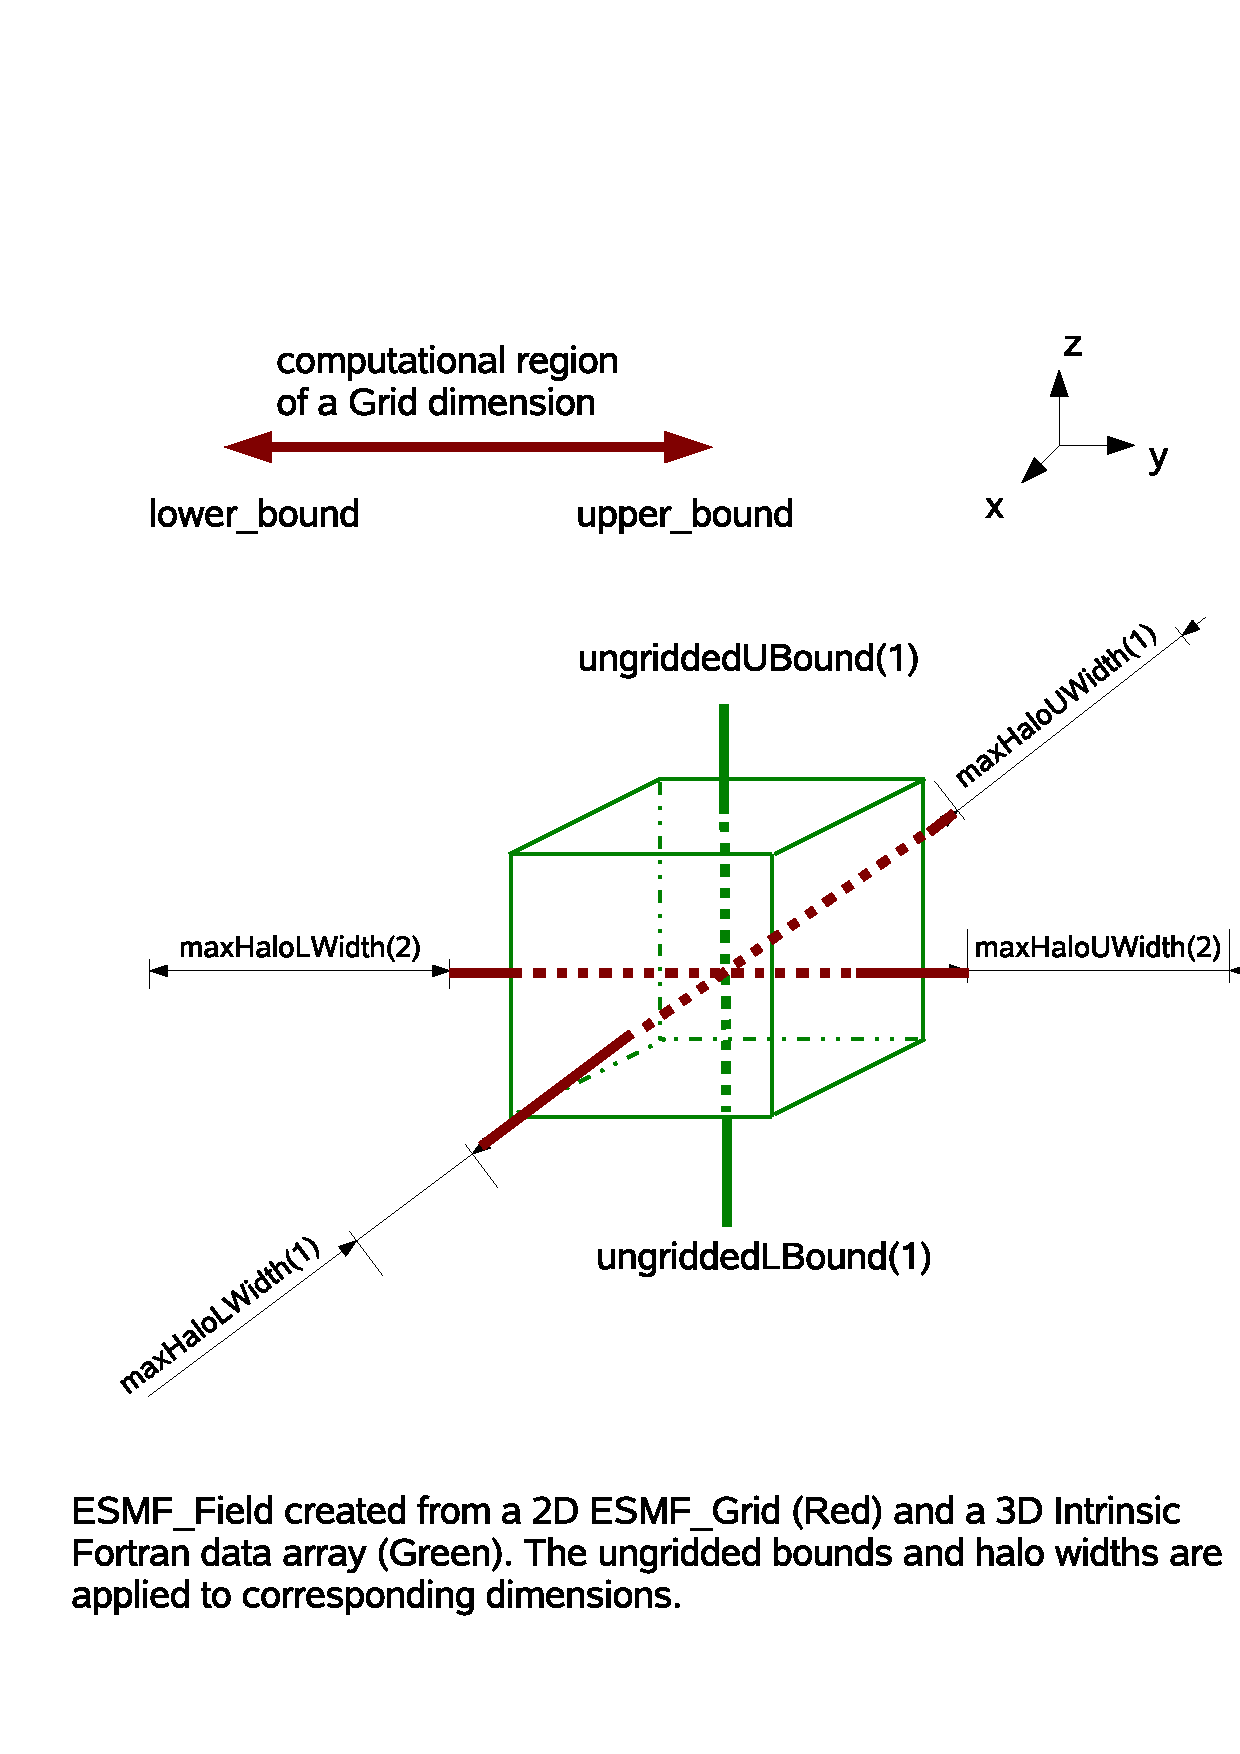
\includegraphics{FieldParameterSetup}}
  \caption{Field dimension configuration from Grid, halos, and Fortran data array.}
  \label{fig:fieldparameter}
  \end{figure}
  \end{center}
    
    The {\tt ESMF\_FieldCreate()} interface supports creating a Field from a Grid and a
    Fortran array padded with halos on the distributed dimensions of the Fortran
    array. Using this technique one can avoid passing non-contiguous Fortran array
    slice to FieldCreate. It guarantees the same exclusive region,
    and by using halos, it also defines a bigger total region to contain 
    the entire contiguous memory block of the Fortran array.
  
    The elements of totalLWidth and totalUWidth are applied in the order
    distributed dimensions appear in the Fortran array. By definition, 
    totalLWidth and totalUWidth are 1 dimensional arrays of non-negative 
    integer values. The size of haloWidth arrays is equal to the number of distributed
    dimensions of the Fortran array, which is also equal to the number of
    distributed dimensions of the Grid used in the Field creation.
  
    Because the order of totalWidth (representing both totalLWidth and
    totalUWidth) element is applied to the order distributed dimensions
    appear in the Fortran array dimensions, it's quite simple to compute
    the shape of distributed dimensions of the Fortran array. They are done
    in a similar manner when applying ungriddedLBound and ungriddedUBound 
    to ungridded dimensions of the Fortran array defined by rule 2.
  
    Assume we have the mapping from the dimension index of totalWidth
    to the dimension index of Fortran array, called mhw2fa; and we also
    have the mapping from dimension index of Fortran array to dimension
    index of the Grid, called fa2g. The shape of
    distributed dimensions of a Fortran array can be computed by rule 4: 
   
    \begin{verbatim}
  
    (4) fa_shape(mhw2fa(k)) = exclusiveCount(fa2g(mhw2fa(k)) + 
                              totalUWidth(k) + totalLWidth(k)
                          k = 1...size(totalWidth) 
  
    \end{verbatim}
    
    This rule may seem confusing but algorithmically the computation
    can be done by the following pseudocode:
  
    \begin{verbatim}
  
    fa_index = 1
    do i = 1, farray_rank
       if i-th dimension of Fortran array is distributed
           fa_shape(i) = exclusiveCount(fa2g(i)) + 
                         totalUWidth(fa_index) + totalLWidth(fa_index)
           fa_index = fa_index + 1
       endif
    enddo
  
    \end{verbatim}
  
    The only complication then is to figure out the mapping from Fortran
    array dimension index to Grid dimension index. This process can
    be done by computing the reverse mapping from Field to Grid.
  
    Typically, we don't have to consider these complications if the following
    conditions are met: 1) All Grid dimensions are distributed. 2) DistGrid
    in the Grid has a dimension index mapping to the Grid in the form of 
    natural order (/1,2,3,.../). This natural order mapping is the
    default mapping between various objects throughout ESMF. 3) Grid to Field
    mapping is in the form of natural order, i.e. default mapping. These
    seem like a lot of conditions but they are the default case in the interaction
    among DistGrid, Grid, and Field. When these conditions are met, which
    is typically true, the shape of distributed dimensions of Fortran array
    follows rule 5 in a simple form:
  
    \begin{verbatim}
  
    (5) fa_shape(k) = exclusiveCount(k) + 
                      totalUWidth(k) + totalLWidth(k) 
                  k = 1...size(totalWidth)
  
    \end{verbatim}
  
    Let's examine an example on how to apply rule 5. Suppose we have a
    5D array and a 3D Grid that has its first 3 dimensions mapped to the first
    3 dimensions of the Fortran array. totalLWidth=(/1,2,3/), 
    totalUWidth=(/7,9,10/), then by rule 5, the following pseudo code
    can be used to compute the shape of the first 3 dimensions of the Fortran
    array. The shape of the remaining two ungridded dimensions can be
    computed according to rule 2.
  
    \begin{verbatim}
  
    do k = 1, 3
        fa_shape(k) = exclusiveCount(k) + 
                      totalUWidth(k) + totalLWidth(k)) 
    enddo
  
    \end{verbatim}
  
    Suppose now gridToFieldMap=(/2,3,4/) instead which says
    the first dimension of Grid maps to the 2nd dimension of Field (or 
    Fortran array) and so on and so forth, we can obtain a more general form 
    of rule 5 by introducing first\_distdim\_index shift when Grid to Field
    map (gridToFieldMap) is in the form of (/a,a+1,a+2.../).
  
    \begin{verbatim}
  
    (6) fa_shape(k+first_distdim_index-1) = exclusiveCount(k) +
                                            totalUWidth(k) + totalLWidth(k)
                                        k = 1...size(totalWidth)
  
    \end{verbatim}
  
    It's obvious that first\_distdim\_index=a. If the first dimension of the Fortran
    array is distributed, then rule 6 degenerates into rule 5, which is
    the typical case.
  
    Back to our example creating a 3D Field from a 2D Grid and a 3D intrinsic
    Fortran array, we will use the Grid created from previous example
    that satisfies condition 1 and 2. We'll also use a simple gridToFieldMap
    (1,2) which is the default mapping that satisfies condition 3. 
    First we use rule 5 to compute
    the shape of distributed dimensions then we use rule 2 to compute the shape
    of the ungridded dimensions. 
%/////////////////////////////////////////////////////////////

 \begin{verbatim}
    gridToFieldMap2d(1) = 1
    gridToFieldMap2d(2) = 2
    totalLWidth2d(1) = 3
    totalLWidth2d(2) = 4
    totalUWidth2d(1) = 3
    totalUWidth2d(2) = 5
    do k = 1, 2
        fa_shape(k) = gec(k) + totalLWidth2d(k) + totalUWidth2d(k)
    end do
    fa_shape(3) = 7          ! 9-3+1
    allocate(farray3d(fa_shape(1), fa_shape(2), fa_shape(3)))
    field = ESMF_FieldCreate(grid, farray3d, ESMF_INDEX_DELOCAL, &
        ungriddedLBound=(/3/), ungriddedUBound=(/9/), &
        totalLWidth=totalLWidth2d, totalUWidth=totalUWidth2d, &
        gridToFieldMap=gridToFieldMap2d, &
        rc=rc)
    if (rc /= ESMF_SUCCESS) call ESMF_Finalize(endflag=ESMF_END_ABORT)
 
\end{verbatim}
 
%/////////////////////////////////////////////////////////////

  \subsubsection{Create a Field from a LocStream, typekind, and rank}
  \label{sec:field:usage:create_locs_tkr}
   
   In this example, an {\tt ESMF\_Field} is created from an {\tt ESMF\_LocStream} 
   and typekind/rank.
   The location stream object is uniformly distributed
   in a 1 dimensional space on 4 DEs. The rank is 1 dimensional. 
   Please refer to LocStream examples section for more information on LocStream creation.
   
%/////////////////////////////////////////////////////////////

 \begin{verbatim}

    locs = ESMF_LocStreamCreate(minIndex=1, maxIndex=16, rc=rc)
    if (rc /= ESMF_SUCCESS) call ESMF_Finalize(endflag=ESMF_END_ABORT)

    field = ESMF_FieldCreate(locs, typekind=ESMF_TYPEKIND_I4, &
        rc=rc)
    if (rc /= ESMF_SUCCESS) call ESMF_Finalize(endflag=ESMF_END_ABORT)

 
\end{verbatim}
 
%/////////////////////////////////////////////////////////////

  \subsubsection{Create a Field from a LocStream and arrayspec}
  \label{sec:field:usage:create_locs_arrayspec}
   
   In this example, an {\tt ESMF\_Field} is created from an {\tt ESMF\_LocStream} 
   and an {\tt ESMF\_Arrayspec}.
   The location stream object is uniformly distributed
   in a 1 dimensional space on 4 DEs. The arrayspec is 1 dimensional. 
   Please refer to LocStream examples section for more information on LocStream creation.
   
%/////////////////////////////////////////////////////////////

 \begin{verbatim}

    locs = ESMF_LocStreamCreate(minIndex=1, maxIndex=16, rc=rc)
    if (rc /= ESMF_SUCCESS) call ESMF_Finalize(endflag=ESMF_END_ABORT)

    call ESMF_ArraySpecSet(arrayspec, 1, ESMF_TYPEKIND_I4, rc=rc)
    if (rc /= ESMF_SUCCESS) call ESMF_Finalize(endflag=ESMF_END_ABORT)

    field = ESMF_FieldCreate(locs, arrayspec, &
        rc=rc)
    if (rc /= ESMF_SUCCESS) call ESMF_Finalize(endflag=ESMF_END_ABORT)

 
\end{verbatim}
 
%/////////////////////////////////////////////////////////////

  \subsubsection{Create a Field from a Mesh, typekind, and rank}
  \label{sec:field:usage:create_mesh_tkr}
   
   In this example, an {\tt ESMF\_Field} is created from an {\tt ESMF\_Mesh} 
   and typekind/rank.
   The mesh object is on a Euclidean surface that is partitioned to a 2x2 rectangular
   space with 4 elements and 9 nodes. The nodal space is represented by
   a distgrid with 9 indices. A Field is created on locally owned nodes on each PET.
   Therefore, the created Field has 9 data points globally.
   The mesh object can be represented by the picture
   below. For more information on Mesh creation, please see Section~\ref{sec:mesh:usage:meshCreation}.
   \begin{verbatim}
                Mesh Ids
  
    2.0   7 ------- 8 -------- 9
          |         |          |
          |    3    |    4     |
          |         |          |
    1.0   4 ------- 5 -------- 6
          |         |          |
          |    1    |    2     |
          |         |          |
    0.0   1 ------- 2 -------- 3
  
         0.0       1.0        2.0 
  
        Node Ids at corners
        Element Ids in centers
   
  
               Mesh Owners
  
    2.0   2 ------- 2 -------- 3
          |         |          |
          |    2    |    3     |
          |         |          |
    1.0   0 ------- 0 -------- 1
          |         |          |
          |    0    |    1     |
          |         |          |
    0.0   0 ------- 0 -------- 1
  
         0.0       1.0        2.0 
  
        Node Owners at corners
        Element Owners in centers
  \end{verbatim} 
   
%/////////////////////////////////////////////////////////////

 \begin{verbatim}
      ! Create Mesh structure in 1 step
      mesh=ESMF_MeshCreate(parametricDim=2,spatialDim=2, &
             nodeIds=nodeIds, nodeCoords=nodeCoords, &
             nodeOwners=nodeOwners, elementIds=elemIds,&
             elementTypes=elemTypes, elementConn=elemConn, &
             rc=rc)
      if (rc /= ESMF_SUCCESS) call ESMF_Finalize(endflag=ESMF_END_ABORT)

      ! Field is created on the 1 dimensional nodal distgrid. On
      ! each PET, Field is created on the locally owned nodes.
      field = ESMF_FieldCreate(mesh, typekind=ESMF_TYPEKIND_I4, rc=rc)
      if (rc /= ESMF_SUCCESS) call ESMF_Finalize(endflag=ESMF_END_ABORT)
 
\end{verbatim}
 
%/////////////////////////////////////////////////////////////

  \subsubsection{Create a Field from a Mesh and arrayspec}
  \label{sec:field:usage:create_mesh_arrayspec}
   
   In this example, an {\tt ESMF\_Field} is created from an {\tt ESMF\_Mesh} 
   and an {\tt ESMF\_Arrayspec}.
   The mesh object is on a Euclidean surface that is partitioned to a 2x2 rectangular
   space with 4 elements and 9 nodes. The nodal space is represented by
   a distgrid with 9 indices. Field is created on locally owned nodes on each PET.
   Therefore, the created Field has 9 data points globally.
   The mesh object can be represented by the picture
   below. For more information on Mesh creation, please see Section~\ref{sec:mesh:usage:meshCreation}.
   
%/////////////////////////////////////////////////////////////

 \begin{verbatim}
      ! Create Mesh structure in 1 step
      mesh=ESMF_MeshCreate(parametricDim=2,spatialDim=2, &
             nodeIds=nodeIds, nodeCoords=nodeCoords, &
             nodeOwners=nodeOwners, elementIds=elemIds,&
             elementTypes=elemTypes, elementConn=elemConn, &
             rc=rc)
      if (rc /= ESMF_SUCCESS) call ESMF_Finalize(endflag=ESMF_END_ABORT)

      call ESMF_ArraySpecSet(arrayspec, 1, ESMF_TYPEKIND_I4, rc=rc)
      if (rc /= ESMF_SUCCESS) call ESMF_Finalize(endflag=ESMF_END_ABORT)

      ! Field is created on the 1 dimensional nodal distgrid. On
      ! each PET, Field is created on the locally owned nodes.
      field = ESMF_FieldCreate(mesh, arrayspec, rc=rc)
      if (rc /= ESMF_SUCCESS) call ESMF_Finalize(endflag=ESMF_END_ABORT)
 
\end{verbatim}
 
%/////////////////////////////////////////////////////////////

  \subsubsection{Create a Field from a Mesh and an Array}
  \label{sec:field:usage:create_mesh_array}
   
   In this example, an {\tt ESMF\_Field} is created from an {\tt ESMF\_Mesh} 
   and an {\tt ESMF\_Array}. The mesh object is created in the previous example and
   the array object is retrieved from the field created in the previous example too.
   
%/////////////////////////////////////////////////////////////

 \begin{verbatim}
    call ESMF_MeshGet(mesh, nodalDistgrid=distgrid, rc=rc)
    if (rc /= ESMF_SUCCESS) call ESMF_Finalize(endflag=ESMF_END_ABORT)
    array = ESMF_ArrayCreate(distgrid=distgrid, arrayspec=arrayspec, rc=rc)
    if (rc /= ESMF_SUCCESS) call ESMF_Finalize(endflag=ESMF_END_ABORT)
    ! query the array from the previous example
    call ESMF_FieldGet(field, array=array, rc=rc)
    if (rc /= ESMF_SUCCESS) call ESMF_Finalize(endflag=ESMF_END_ABORT)
    ! create a Field from a mesh and an array
    field1 = ESMF_FieldCreate(mesh, array, rc=rc)
    if (rc /= ESMF_SUCCESS) call ESMF_Finalize(endflag=ESMF_END_ABORT)
 
\end{verbatim}
 
%/////////////////////////////////////////////////////////////

  \subsubsection{Create a Field from a Mesh and an ArraySpec with optional features}
  \label{sec:field:usage:createMeshArrayspecOpt}
  
   In this example, an {\tt ESMF\_Field} is created from an {\tt ESMF\_Mesh}
   and an {\tt ESMF\_ArraySpec}. The mesh object is created in the previous example.
   The Field is also created with optional arguments such as ungridded dimensions
   and dimension mapping.
  
   In this example, the mesh is mapped to the 2nd dimension of the
   {\tt ESMF\_Field}, with its first dimension being the ungridded dimension with bounds 1,3.
   
%/////////////////////////////////////////////////////////////

 \begin{verbatim}
    call ESMF_ArraySpecSet(arrayspec, 2, ESMF_TYPEKIND_I4, rc=rc)
    field = ESMF_FieldCreate(mesh, arrayspec=arrayspec, gridToFieldMap=(/2/), &
        ungriddedLBound=(/1/), ungriddedUBound=(/3/), rc=rc)
    if (rc /= ESMF_SUCCESS) call ESMF_Finalize(endflag=ESMF_END_ABORT)
 
\end{verbatim}

%...............................................................
\setlength{\parskip}{\oldparskip}
\setlength{\parindent}{\oldparindent}
\setlength{\baselineskip}{\oldbaselineskip}
